\section{Results}
% CONTENT GOAL: Report all completed/error counts next to category-macro scores and keep internal mode comparisons bounded.
% VERIFIED FACT: Development Full Omni=\DevelopmentFullOverall, Retrieval-only=\DevelopmentRetrievalOverall, No Memory=\DevelopmentNoMemoryOverall.
% VERIFIED FACT: Formal completed 248/250 with two errors and Overall=\FormalOverall.
% VERIFIED FACT: Comparison Full Omni=\ComparisonFullOverall; Retrieval-only is 69/70 at \ComparisonRetrievalOverall; No Memory=\ComparisonNoMemoryOverall.
% EVIDENCE: docs/omni-context-paper-evidence-v1/metrics/
% FORBIDDEN: Call the mode comparison a strict component ablation.

\begin{table*}[t]
\centering
\caption{Version-locked internal benchmark results. Completed and error counts are never suppressed.}
\label{tab:main-results}
\begin{tabular}{llrrr}
\toprule
Evaluation & Mode & Completed & Errors & Overall \\
\midrule
Targeted-7 & Full Omni & 7/7 & 0 & 0.840868 \\
Development-35 & Full Omni & 35/35 & 0 & 0.884842 \\
Development-35 & Retrieval-only & 35/35 & 0 & 0.563853 \\
Development-35 & No Memory & 35/35 & 0 & 0.366713 \\
Formal-250 & Full Omni & 248/250 & 2 & 0.866546 \\
Comparison-70 & Full Omni & 70/70 & 0 & 0.870698 \\
Comparison-70 & Retrieval-only & 69/70 & 1 & 0.552346 \\
Comparison-70 & No Memory & 70/70 & 0 & 0.364683 \\
\bottomrule
\end{tabular}
\begin{minipage}{0.96\textwidth}\footnotesize
Formal-250 Overall is computed over successfully completed records using the benchmark's category-macro definition. These mode comparisons are not strict component ablations. All evaluations shown here are internal Synthetic Curated Benchmark results; external held-out validity has not been established.
\end{minipage}
\end{table*}

\begin{table*}[t]
\centering\small
\caption{Category-macro results. The mode delta is Comparison-70 Full Omni minus the stronger of Retrieval-only and No Memory.}
\label{tab:category-results}
\begin{tabular}{lrrrrrr}
\toprule
Category & Dev Full & Formal Full & Comp Full & Comp Ret. & Comp No Mem. & $\Delta$ \\
\midrule
Cognitive Continuity & 0.916667 & 0.936667 & 0.956667 & 0.616667 & 0.500000 & 0.340000 \\
Memory Evolution & 0.856746 & 0.852866 & 0.897963 & 0.407130 & 0.208333 & 0.490833 \\
Conflict Resolution & 0.833333 & 0.812500 & 0.788889 & 0.327160 & 0.222222 & 0.461729 \\
Cross-Agent Transfer & 1.000000 & 1.000000 & 0.994444 & 0.755556 & 0.500000 & 0.238888 \\
Human-like Forgetting & 0.927778 & 0.884722 & 0.886111 & 0.669444 & 0.416667 & 0.216667 \\
Proactive Insight & 0.875000 & 0.770833 & 0.800000 & 0.487500 & 0.400000 & 0.312500 \\
Decision Quality & 0.784370 & 0.808235 & 0.770815 & 0.602963 & 0.305556 & 0.167852 \\
\bottomrule
\end{tabular}
\begin{minipage}{0.98\textwidth}\footnotesize
Values are benchmark category means, not scenario-weighted averages. Development and Formal baseline-by-category values are not invented; only available verified columns are shown.
\end{minipage}
\end{table*}


\begin{figure}[t]
  \centering
  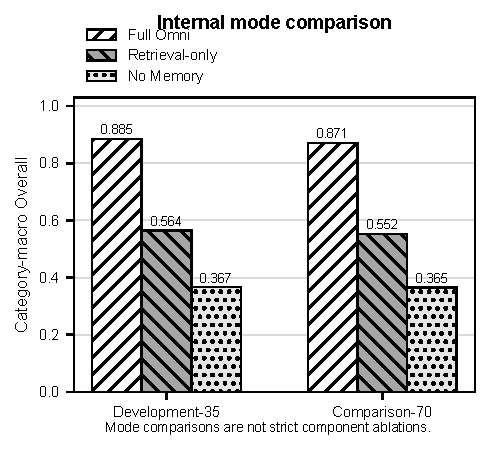
\includegraphics[width=\columnwidth]{../figures/overall-comparison.pdf}
  \caption{Internal Development-35 and Comparison-70 mode results.}
  \label{fig:overall-comparison}
\end{figure}

\begin{figure*}[t]
  \centering
  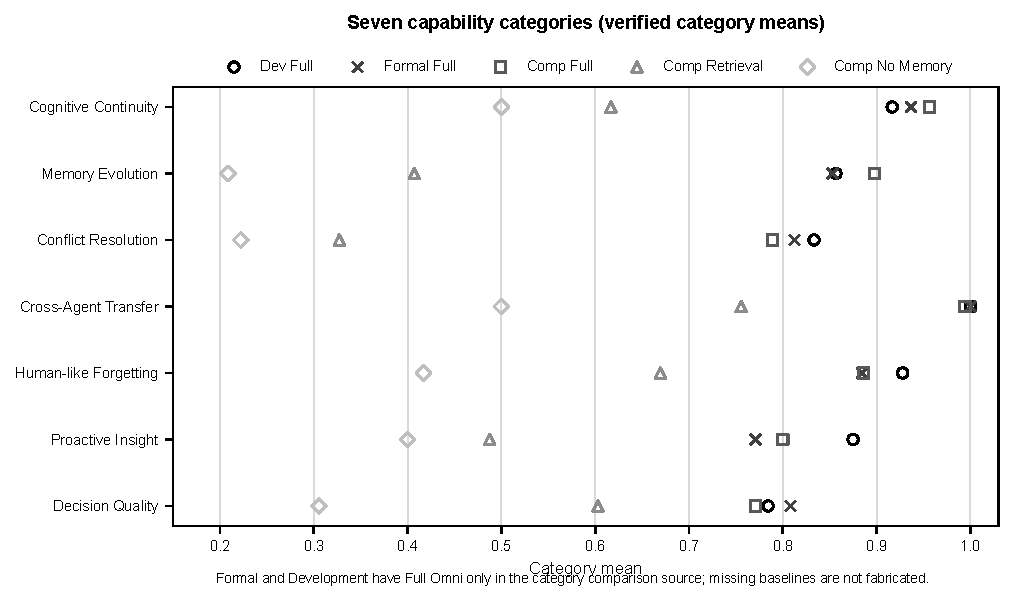
\includegraphics[width=\textwidth]{../figures/category-comparison.pdf}
  \caption{Verified category means. Missing Development/Formal baselines are not fabricated.}
  \label{fig:category-comparison}
\end{figure*}

\TODO{Author interpretation required.}

\begin{table*}[t]
\centering\small
\caption{External held-out evaluation status. No score is available or implied.}
\label{tab:external-heldout}
\begin{tabularx}{\textwidth}{p{0.20\textwidth}p{0.20\textwidth}X p{0.10\textwidth}}
\toprule
Benchmark & Adapter fixtures & Preregistration & Formal result \\
\midrule
LongMemEval-S cleaned & PASS (12 fictional records) & Adapter locked; dataset authorization pending & \textbf{NOT RUN} \\
LoCoMo QA, Conversations 2--10 & PASS (4 fictional QA forms) & Adapter locked; dataset authorization pending & \textbf{NOT RUN} \\
\bottomrule
\end{tabularx}
\end{table*}

